\section{Experiments}

\subsection{Experimental Setup}

We evaluate taxonomy-bearing prompts on a stratified iNat21 subset consisting of
821 species and 8{,}210 images drawn from five broad taxonomic groups (Aves,
Insecta, Plantae, Fungi, Reptilia), the only configuration in our study spanning multiple kingdoms
and therefore the only one permitting evaluation at every Linnaean rank including
kingdom. BioCLIP2 (ViT-L/14, \texttt{hf:imageomics/bioclip-2}) serves as the
primary biological vision--language model, while OpenCLIP ViT-L/14
(\texttt{laion2b\_s32b\_b82k}) is included as a general-domain reference baseline.
All experiments use frozen models without additional fine-tuning. For the
embedding-geometry analyses, each image embedding is fused with its per-sample
prompt embedding by $L_2$-normalizing both modalities and concatenating them;
zero-shot classification instead assigns each image to the nearest per-class text
prototype by cosine similarity (no concatenation). Since the fused text vector is
identical for all images of the same species, rank-level geometry partly reflects
text-vector structure; the latent taxonomy probe (Section~\ref{sec:latent}),
operating on image embeddings alone, serves as a control for this confound.
Reported numbers are means over 5 seeds. To test whether our conclusions generalize
beyond a single benchmark, we additionally replicate the full protocol on the Rare
Species dataset (400 species, 11{,}983 images; Section~\ref{sec:rare}).

We evaluate five prompt conditions introduced in Section~\ref{sec:method}: C0 (flat species
labels), C1 (hierarchy-preserving taxonomy prompts), C2 (random-token hierarchy;
slot format preserved, vocabulary replaced with placeholders), C3 (wrong-taxonomy
hierarchy; slot format preserved, taxonomic coherence destroyed), and C4
(bag-of-words taxonomy; same tokens, order destroyed). This counterfactual design
lets us isolate the \emph{content} of the taxonomy text from its \emph{structure}.
Our evaluation considers both downstream classification performance and
embedding-space organization.

\subsection{Species-Level Performance}

We first investigate whether taxonomy-bearing prompts improve species-level
classification accuracy.

\begin{table}[t]
\centering
\caption{Zero-shot top-1 classification accuracy (\%) across prompt conditions.
C0--C4 build per-class text prototypes from each prompt variant.}
\label{tab:accuracy}
\begin{tabular}{lcc}
\hline
Condition & BioCLIP2 & OpenCLIP \\
\hline
C0 (flat)             & \textbf{94.29} & 11.33 \\
C1 (hierarchy)        & 93.73 & 10.37 \\
C2 (random-token)     & 46.43 & 8.19 \\
C3 (wrong-taxonomy)   & 35.05 & 3.25 \\
C4 (bag-of-words)     & 90.15 & \textbf{11.35} \\
\hline
\end{tabular}
\end{table}

Table~\ref{tab:accuracy} shows that hierarchy-preserving prompts do not outperform
flat species labels in species-level classification: for BioCLIP2 the strongest
accuracy is obtained by the flat-label baseline (C0, 94.29\%), with the
hierarchical prompt marginally lower (C1, 93.73\%). This observation suggests that
the primary role of hierarchy is not direct classification improvement.

In contrast, both the random-token (C2, 46.43\%) and wrong-taxonomy (C3, 35.05\%)
conditions exhibit substantial degradation, indicating that BioCLIP2 remains highly
sensitive to taxonomy-related semantic information. Notably, the bag-of-words
variant (C4) retains 90.15\% accuracy, so destroying \emph{order} alone is far less
damaging than destroying the \emph{tokens} (C2) or the taxonomic \emph{coherence} (C3).

\subsection{Species-Level Representation Geometry}

To determine whether hierarchy alters the structure of the embedding space, we
evaluate species-level geometry using silhouette score, inter-class margin, kNN
purity, and intra-class variance, comparing the flat baseline (C0) against the
hierarchy-preserving prompt (C1).

\begin{table}[t]
\centering
\caption{Species-level geometry metrics (BioCLIP2). Higher is better for
Silhouette, Margin, and Purity; lower is better for Variance.}
\label{tab:species_geometry}
\begin{tabular}{lcccc}
\hline
Condition & Silhouette & Margin & Purity & Variance \\
\hline
C0 & \textbf{0.683} & \textbf{14.91} & \textbf{0.895} & 0.0721 \\
C1 & 0.671 & 14.50 & 0.891 & 0.0721 \\
\hline
\end{tabular}
\end{table}

The species-level geometry results (Table~\ref{tab:species_geometry}) mirror the
classification findings: the flat-label baseline achieves marginally stronger
species-level organization across all four metrics ($\Delta$silhouette $=-0.011$). These differences are small and,
under our statistical protocol, do not survive multiple-comparison correction
(Section~\ref{sec:robustness}). The takeaway is therefore not that hierarchy
\emph{hurts} species discrimination, but that it does not \emph{help} it---the
species representation is already near-saturated under flat labels
(silhouette $0.68$, kNN purity $0.90$). These findings indicate that hierarchical
prompts do not primarily act by improving species discrimination.

\subsection{Rank-Level Taxonomic Organization}
\label{sec:rank}

We next investigate whether hierarchy-bearing prompts influence higher-order
biological organization. For each condition, embeddings are grouped according to
taxonomic rank and evaluated using silhouette score.

\begin{table}[t]
\centering
\caption{Rank-level silhouette scores (C0 vs C1). $\Delta$ is C1$-$C0; positive
values indicate hierarchy improves organization at that rank. Kingdom and phylum
comprise only 3--5 clusters in iNat21, so their silhouette estimates carry higher
variance than intermediate ranks.}
\label{tab:rank_geometry}
\begin{tabular}{lcccc}
\hline
 & \multicolumn{2}{c}{BioCLIP2} & \multicolumn{2}{c}{OpenCLIP} \\
Rank & C0 & C1 & C0 & C1 \\
\hline
Kingdom & 0.049 & \textbf{0.053} & 0.069 & \textbf{0.226} \\
Phylum  & 0.027 & \textbf{0.032} & 0.005 & \textbf{0.144} \\
Class   & 0.001 & \textbf{0.011} & 0.011 & \textbf{0.192} \\
Order   & 0.026 & \textbf{0.035} & 0.012 & \textbf{0.110} \\
Family  & 0.252 & \textbf{0.272} & \textbf{0.172} & 0.139 \\
Genus   & 0.591 & \textbf{0.609} & \textbf{0.488} & 0.268 \\
Species & \textbf{0.683} & 0.671 & \textbf{0.452} & 0.226 \\
\hline
\end{tabular}
\end{table}

Unlike the species-level results, a clear directional pattern emerges
(Table~\ref{tab:rank_geometry}). For BioCLIP2, hierarchy-preserving prompts improve
organization at \emph{every} rank from kingdom through genus, with the largest
absolute gains at the intermediate family ($+0.020$) and genus ($+0.018$) ranks,
and reverse sign only at the species rank ($-0.011$). This sign-flip---C1 dominant
at coarse ranks, C0 dominant only at the species rank---suggests that
hierarchy-bearing prompts encourage embeddings to respect broader biological
relationships rather than improving species-level separation.

These findings support the hypothesis that taxonomy-bearing prompts function as
\emph{taxonomic organizers} rather than accuracy boosters. The OpenCLIP columns
foreshadow Section~\ref{sec:openclip}: the general-domain model shows strong gains
only at the coarsest ranks (kingdom--order) and collapses from family downward,
whereas BioCLIP2 sustains positive gains through genus.

Figure~\ref{fig:delta_silhouette} plots $\Delta$silhouette
$(\mathrm{C1}-\mathrm{C0})$ across ranks for both models on both datasets,
summarizing the central result of this study at a glance: the sign-flip at species,
BioCLIP2's positive gains sustained through genus, and OpenCLIP's strong coarse-rank
gains followed by collapse from family downward---all recurring on iNat21 and Rare
Species alike.

\begin{figure}[t]
  \centering
  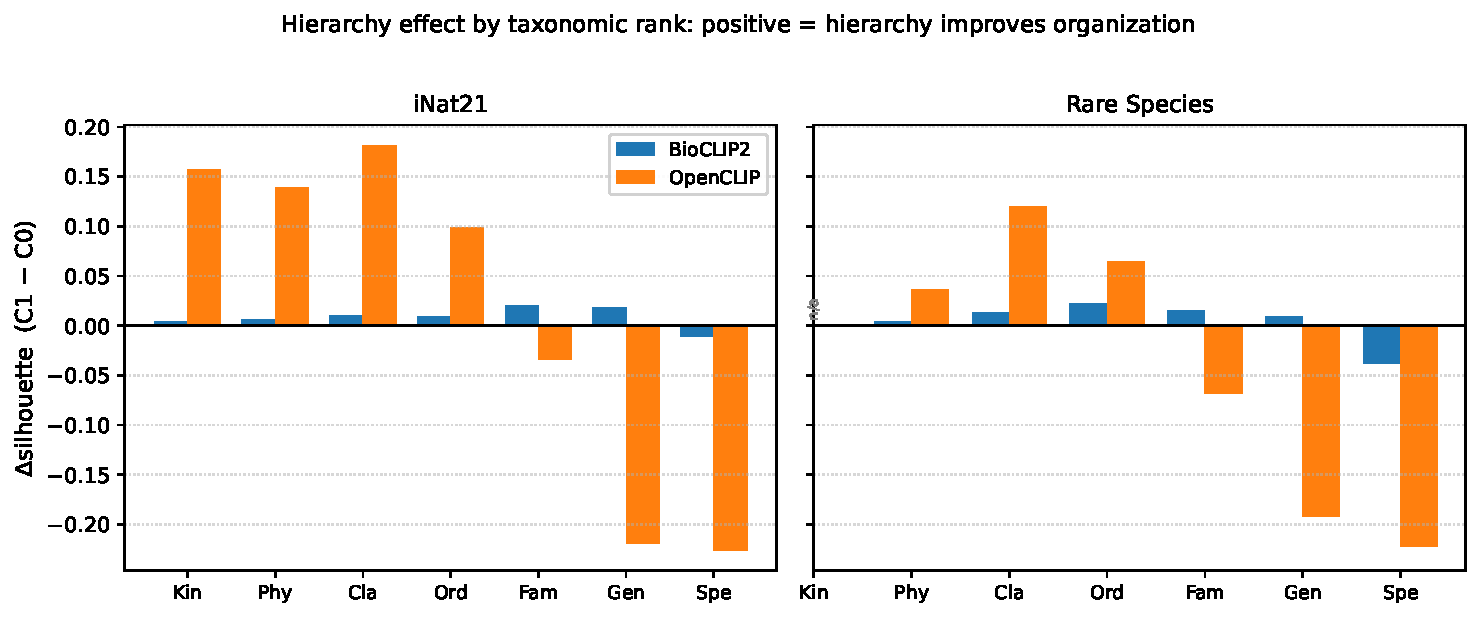
\includegraphics[width=\linewidth]{figures/delta_silhouette_by_rank.pdf}
  \caption{Per-rank $\Delta$silhouette $(\mathrm{C1}-\mathrm{C0})$ for BioCLIP2 and
  OpenCLIP, on iNat21 (left) and Rare Species (right). Positive bars mean
  hierarchy-preserving prompts improve organization at that rank. BioCLIP2 stays
  positive through genus and flips sign only at species; OpenCLIP gains only at the
  coarsest ranks and collapses from family downward. Kingdom is degenerate on Rare
  Species (single kingdom) and marked \emph{n/a}. The pattern is consistent across
  both datasets.}
  \label{fig:delta_silhouette}
\end{figure}

\subsection{Latent Taxonomy Probe}
\label{sec:latent}

If hierarchy merely \emph{added} taxonomic information through text, we would not
expect that information to already be present without any text. We therefore probe
the image embeddings alone: we compute the silhouette of the image embeddings under
the true species-level grouping and compare it against the distribution obtained
from 50 random label permutations, reporting a $z$-score.

\begin{table}[t]
\centering
\caption{Latent taxonomy probe on image-only embeddings. ``Random $\mu$'' is the
mean silhouette over 50 label permutations.}
\label{tab:latent}
\begin{tabular}{lccc}
\hline
Model & Real silhouette & Random $\mu$ & $z$-score \\
\hline
BioCLIP2 & 0.370 & $-0.146$ & \textbf{180.9} \\
OpenCLIP & $-0.017$ & $-0.182$ & 50.7 \\
\hline
\end{tabular}
\end{table}

Both models place real taxonomic structure far outside the permutation null
($z \ge 50$), and BioCLIP2's signal is $\sim$3.6$\times$ stronger than OpenCLIP's
(Table~\ref{tab:latent}). Taxonomic organization is thus already \emph{latent} in
the image embeddings before any text is attached. This reframes the role of
hierarchy-bearing prompts: they do not teach taxonomy so much as surface a structure
the visual encoder already carries---consistent with the organizer interpretation of
Section~\ref{sec:rank}.

\subsection{Counterfactual Prompt Ablation}
\label{sec:ablation}

To disentangle semantic enrichment from hierarchical organization, we compare
hierarchy-preserving prompts against the controlled perturbation variants.

\begin{table}[t]
\centering
\caption{Counterfactual prompt ablation (BioCLIP2). $\Delta$sil. is the silhouette
drop relative to C0. Conditions are ordered by increasing damage.}
\label{tab:ablation}
\begin{tabular}{lcccc}
\hline
Condition & Silhouette & Margin & Variance & $\Delta$sil. vs C0 \\
\hline
C0 (flat)            & 0.683 & 14.91 & 0.072 & --- \\
C1 (hierarchy)       & 0.671 & 14.50 & 0.072 & $-0.011$ \\
C2 (random-token)    & 0.596 & 10.75 & 0.072 & $-0.087$ \\
C4 (bag-of-words)    & 0.552 & 11.45 & 0.100 & $-0.131$ \\
C3 (wrong-taxonomy)  & 0.301 & 8.03  & 0.205 & $-0.381$ \\
\hline
\end{tabular}
\end{table}

The random-token (C2) and wrong-taxonomy (C3) conditions degrade both performance
and representation quality (Table~\ref{tab:ablation}), confirming the importance of
taxonomy-related information. The decisive comparison is between C2 and C3. Both
perturb the taxonomy text, but C2 fills the upper-rank slots with meaningless
placeholder tokens while preserving the slot format, whereas C3 fills the same
slots with real taxonomy labels drawn from other species, destroying taxonomic
coherence while retaining both the slot format and lexical authenticity. C3 degrades
the silhouette $4.4\times$ more than C2 ($-0.381$ vs $-0.087$): destroying
taxonomic coherence (correct species-to-rank associations) is far more damaging
than eliminating token meaningfulness alone. A complementary comparison---C1 vs C4,
which share nearly identical tokens but differ in whether rank order is
preserved---points the same way: C4 is weaker than C1 ($0.552$ vs $0.671$).

This result indicates that the benefit of hierarchy cannot be explained by semantic
enrichment alone; hierarchical \emph{organization} contributes independently to
representation quality. The geometric ordering of damage---vocabulary $<$ order $<$
coherence---is consistent across both models. Note that this geometric ordering
differs from the accuracy ordering in Table~\ref{tab:accuracy}, where bag-of-words
(C4) is the \emph{least} damaging variant ($90.15\%$, vs.\ $46.43\%$ for C2): because
C4 leaves the exact species token intact, nearest-prototype classification still
succeeds even though the scrambled order degrades the embedding geometry more than
token replacement does. The two metrics therefore probe different things---token
presence for classification, rank coherence for geometry---and the coherence-dominant
ordering (C3 worst) holds under both.

\subsection{Statistical Robustness and Limitations}
\label{sec:robustness}

We assess robustness with paired permutation tests (B$=$1000, Bonferroni
$\alpha = 0.01/6$) and bootstrap confidence intervals over seeds. We report a
methodological caveat transparently. Because per-seed stochasticity was injected as
a very small Gaussian image perturbation ($\sigma = 10^{-3}$), seed-to-seed standard
deviations are on the order of $10^{-7}$, which inflates effect-size estimates and
leaves the C0-vs-C1 species-level differences just short of significance after
correction ($p \approx 0.05$--$0.08$). We therefore do not rest any claim on
$p$-values or Cohen's $d$; the evidence in this paper is the \emph{direction and
cross-condition reproducibility} of effects, not their nominal significance.

What \emph{is} robust under this lens is consistent across conditions, ranks, both
models, and two datasets (Section~\ref{sec:rare}): (i) the rank-level
sign-flip---hierarchy helps at every rank above species and only reverses at
species; (ii) the counterfactual ordering---coherence damage (C3) $\gg$ order
damage (C4) $\gg$ vocabulary damage (C2); and (iii) the latent-taxonomy signal
(Section~\ref{sec:latent}) at $z \ge 33$. The consistency of directional effects
across conditions, ranks, two models, and two independent datasets constitutes the
primary evidence in this paper.

\subsection{OpenCLIP Reference Baseline}
\label{sec:openclip}

Finally, we repeat the same protocol with OpenCLIP ViT-L/14 to determine whether the
hierarchy effect is specific to biological foundation models. Three contrasts stand
out. First, in absolute task terms OpenCLIP is far weaker on this fine-grained
benchmark (zero-shot C0 of 11.3\% vs BioCLIP2's 94.3\%; Table~\ref{tab:accuracy}).
Second, its rank-level response is inconsistent: hierarchy helps strongly at the
coarsest ranks (kingdom--order) but \emph{collapses} from family downward
($\Delta$silhouette $-0.034$ at family, $-0.219$ at genus), whereas BioCLIP2
sustains gains through genus (Table~\ref{tab:rank_geometry}). Third, its latent
taxonomy signal is $3.6\times$ weaker ($z = 50.7$ vs $180.9$;
Table~\ref{tab:latent}).

Taken together, hierarchy-sensitive organization---spanning coarse \emph{and}
intermediate ranks, with strong latent structure---emerges primarily from biological
pretraining rather than being a universal property of vision--language models.

\subsection{Cross-Dataset Replication: Rare Species}
\label{sec:rare}

To test whether the iNat21 findings generalize beyond a single benchmark, we repeat
the full protocol on the Rare Species dataset (\texttt{imageomics/rare-species};
400 species, 11{,}983 images). Both models are run with the identical pipeline used
for iNat21. Unlike iNat21, Rare Species spans multiple phyla but a single kingdom
(Animalia), so the kingdom rank is degenerate and omitted; all other ranks are
evaluated identically.

\begin{table}[t]
\centering
\caption{Rare Species rank-level silhouette scores (C0 vs C1). Kingdom is degenerate
(single kingdom) and omitted. Bold marks the stronger of C0/C1 per model per rank.}
\label{tab:rare_rank}
\begin{tabular}{lcccc}
\hline
 & \multicolumn{2}{c}{BioCLIP2} & \multicolumn{2}{c}{OpenCLIP} \\
Rank & C0 & C1 & C0 & C1 \\
\hline
Phylum  & 0.046 & \textbf{0.050} & 0.003 & \textbf{0.040} \\
Class   & 0.045 & \textbf{0.058} & 0.008 & \textbf{0.127} \\
Order   & 0.180 & \textbf{0.202} & 0.088 & \textbf{0.153} \\
Family  & 0.382 & \textbf{0.397} & \textbf{0.273} & 0.205 \\
Genus   & 0.561 & \textbf{0.570} & \textbf{0.446} & 0.254 \\
Species & \textbf{0.592} & 0.554 & \textbf{0.430} & 0.208 \\
\hline
\end{tabular}
\end{table}

Table~\ref{tab:rare_rank} reproduces the central iNat21 pattern on an independent
dataset. For BioCLIP2 the sign-flip recurs exactly: hierarchy-preserving prompts
improve organization at every measurable rank from phylum through genus and reverse
only at species ($\Delta$silhouette $=-0.038$). OpenCLIP again gains only at the
coarsest ranks (phylum--order) and collapses from family downward ($-0.068$ at
family, $-0.192$ at genus, $-0.222$ at species)---the same early-collapse signature
seen on iNat21 (Table~\ref{tab:rank_geometry}).

\begin{table}[t]
\centering
\caption{Rare Species zero-shot top-1 accuracy (\%) across prompt conditions.}
\label{tab:rare_acc}
\begin{tabular}{lcc}
\hline
Condition & BioCLIP2 & OpenCLIP \\
\hline
C0 (flat)             & \textbf{79.85} & 9.19 \\
C1 (hierarchy)        & 76.19 & 10.06 \\
C2 (random-token)     & 25.68 & 6.70 \\
C3 (wrong-taxonomy)   & 11.02 & 3.22 \\
C4 (bag-of-words)     & 69.77 & \textbf{10.21} \\
\hline
\end{tabular}
\end{table}

The zero-shot accuracy pattern likewise mirrors iNat21 (Table~\ref{tab:rare_acc}).
For BioCLIP2 the flat baseline is strongest (C0 $79.85\%$ vs C1 $76.19\%$),
bag-of-words retains most of the accuracy (C4 $69.77\%$), and token or coherence
corruption collapses it (C2 $25.68\%$, C3 $11.02\%$); OpenCLIP hovers near its
fine-grained floor ($\sim$10\%) across all conditions. As on iNat21, hierarchy does
not improve species-level accuracy, yet destroying taxonomy content sharply
degrades it.

The counterfactual ordering also replicates. On Rare Species the silhouette drop
relative to C0 follows vocabulary $<$ order $<$ coherence for \emph{both} models:
BioCLIP2 C2 $-0.161 <$ C4 $-0.202 <$ C3 $-0.402$ (a $2.5\times$ coherence-vs-vocabulary
gap), and OpenCLIP C2 $-0.111 <$ C4 $-0.224 <$ C3 $-0.375$ ($3.4\times$). Finally,
the latent taxonomy probe again separates the two model families by a wide margin:
BioCLIP2 places real species structure at $z = 234.5$ versus OpenCLIP's $z = 33.0$
($\sim$7$\times$ stronger), echoing the $\sim$3.6$\times$ gap on iNat21
(Table~\ref{tab:latent}). Across two datasets, three rank patterns, and two model
families, the organizer interpretation and the coherence-over-vocabulary ordering
hold consistently.
